% ------------------------------------------------------------------------------
% TYPO3 CMS 6.2 LTS - What's New - Chapter "Introduction" (Russian Version)
%
% @author	Andrey Aksenov <aksenovaa@bk.ru>
% @license	Creative Commons BY-NC-SA 3.0
% @link		http://typo3.org/download/release-notes/whats-new/
% @language	Russian
% ------------------------------------------------------------------------------
% Standard Slide
% ------------------------------------------------------------------------------

\section{Предисловие}
\begin{frame}[fragile]
	\frametitle{Предисловие}

	\begin{center}\huge{Предисловие}\end{center}
	\begin{center}\huge{\color{typo3darkgrey}\textbf{(Краткий обзор)}}\end{center}

\end{frame}

% ------------------------------------------------------------------------------
% TYPO3 CMS 6.2 LTS: The Facts (1)
% ------------------------------------------------------------------------------
\begin{frame}[fragile]
	\frametitle{Предисловие}
	\framesubtitle{TYPO3 CMS 6.2 LTS: только факты}

	\begin{itemize}
		\item Акцент на:

			\begin{itemize}
				\item Простая миграция
				\item Прочный и надежный фундамент
				\item Удобство для пользователей
				\item Современные технологии/совместимость
			\end{itemize}

	\end{itemize}

	\begin{columns}[T]

		\begin{column}{.5\textwidth}
			\begin{itemize}
				\item Ответственный за версию:
				\begin{itemize}
					\item Ernesto Baschny\newline
						ernesto.baschny (at) typo3.org\newline
						Twitter: @baschny
				\end{itemize}
			\end{itemize}
		\end{column}

		\begin{column}{.5\textwidth}
			\begin{figure}
				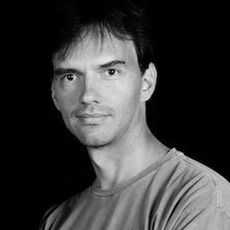
\includegraphics[width=2.6cm,height=2.6cm]{Images/Introduction/ErnestoBaschny.jpg}
			\end{figure}
		\end{column}

	\end{columns}

\end{frame}

% ------------------------------------------------------------------------------
% Standard Slide
% ------------------------------------------------------------------------------

\begin{frame}[fragile]
	% \TabPositions{1.2cm}

	\frametitle{Предисловие}
	\framesubtitle{TYPO3 CMS 6.2 LTS: только факты}

	\begin{itemize}
		\item Дата выхода: 25 марта 2014
		\item Сроки разработки и выхода:
	\end{itemize}

	\begin{figure}
		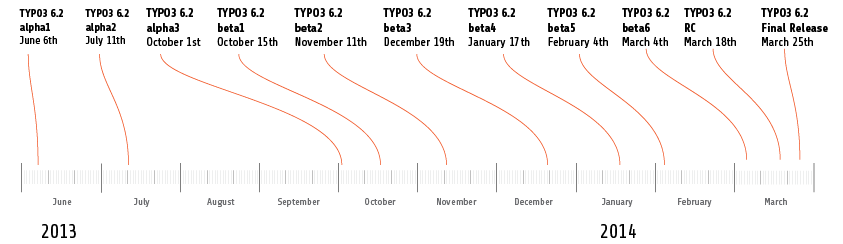
\includegraphics[width=0.99\linewidth]{Images/Introduction/ReleaseTimeline.png}
	\end{figure}

\end{frame}

% ------------------------------------------------------------------------------
% Standard Slide
% ------------------------------------------------------------------------------

\begin{frame}[fragile]
	\frametitle{Предисловие}
	\framesubtitle{TYPO3 CMS 6.2 LTS: только факты}

	\begin{itemize}
		\item Системные требования
		\begin{itemize}
			\item PHP	\tabto{2cm} 5.3.7 - 5.5.x
			\item MySQL	\tabto{2cm} 5.1.x - 5.6.x
		\end{itemize}
	\end{itemize}

	\begin{itemize}
		\item Окончание поддержки: март 2017
		\item TYPO3 CMS 6.2 — это версия \textbf{Long Term Support}\newline(LTS — с долгосрочной поддержкой) (3 года!)
	\end{itemize}

\end{frame}

% ------------------------------------------------------------------------------
% Standard Slide
% ------------------------------------------------------------------------------

\begin{frame}[fragile]
	\frametitle{Предисловие}
	\framesubtitle{TYPO3 CMS 6.2 LTS: только факты}

	\begin{itemize}
		\item Сроки разработки:
	\end{itemize}

	\begin{figure}
		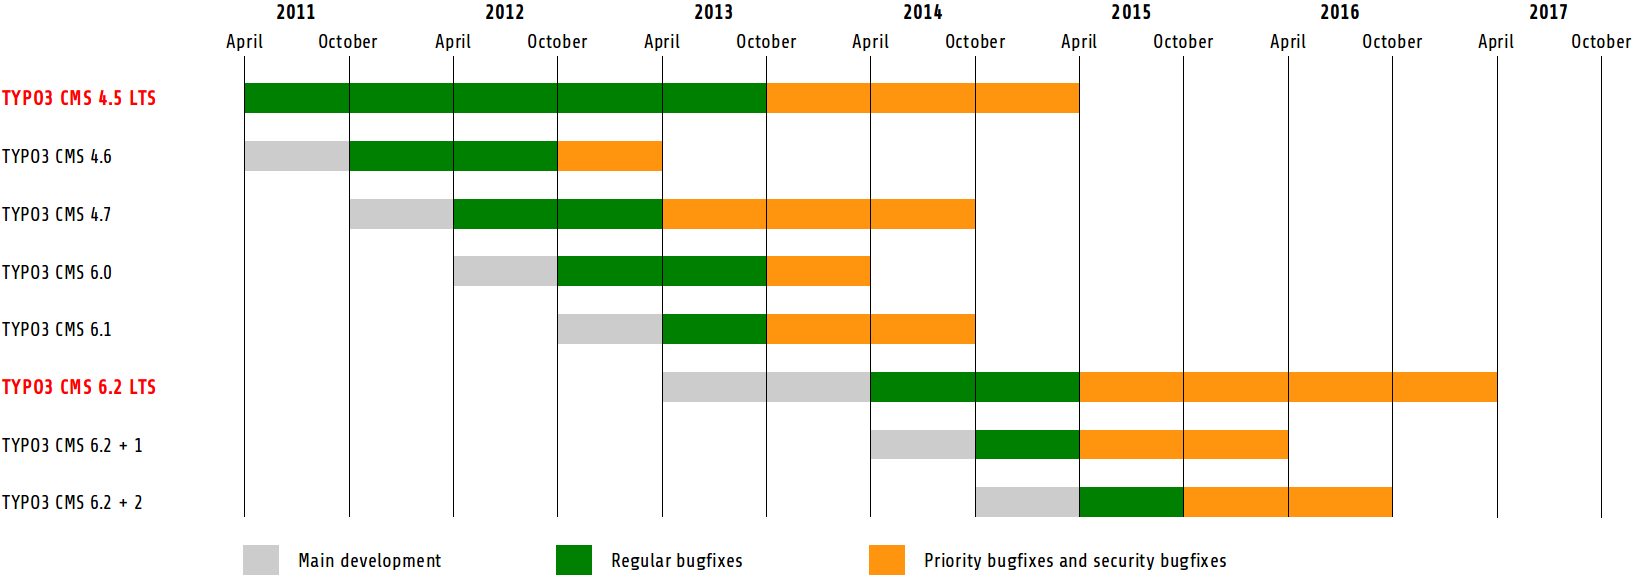
\includegraphics[width=0.99\linewidth]{Images/Introduction/ReleaseAgenda.png}
	\end{figure}

\end{frame}

% ------------------------------------------------------------------------------

